
\subsection*{task 1.7 \\[1ex] getting used to meshgrids (part 2)}

Read image \texttt{portrait.png} into an array \texttt{arrF}. Then ---without using \keyword{for} loops--- create an image array \texttt{arrG} whose content looks like shown below
\begin{figure}[h!]
\begin{center}
\subfloat[\texttt{arrF}]{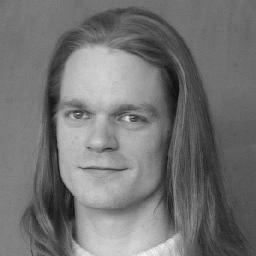
\includegraphics[width=0.45\textwidth]{portrait.png}} \hfill
\subfloat[\texttt{arrG}]{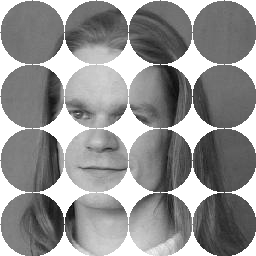
\includegraphics[width=0.45\textwidth]{t1-7.png}}
\end{center}
\end{figure}

\textbf{Note:} the circles in the above figure have a radius of $r = 32$ pixels. Implement your code such that it produces circles of radius $r \in \{ 16, 64 \}$ pixels. \\[1ex]
%%%%%
%%%%%
%%%%% enter your code into the following environment
%%%%%
%%%%%
\begin{python}
# paste your code here

\end{python}
%%%%%
%%%%%
%%%%%
%%%%%
%%%%%



\newpage
Perform runtime measurements for your code and paste your result here. (When implemented ``properly'', your solution should be able to process  \texttt{portrait.png} in only $O(10^{-5})$ seconds \ldots)
\color{blue} \\[1ex]
%%%%%
%%%%%
%%%%% enter your result here
%%%%%
%%%%%
enter your result here \ldots
%%%%%
%%%%%
%%%%%
%%%%%
%%%%%
\color{black}



\vspace{4cm}
Finally, enter your resulting images (for $r \in \{ 16, 64 \}$) here
%%%%%
%%%%%
%%%%% enter your result here, i.e. replace "placeholder.pdf" by the names of the image files you created
%%%%%
%%%%%
\begin{center}

\includegraphics[width=0.45\textwidth]{placeholder.pdf} \hfill

\includegraphics[width=0.45\textwidth]{placeholder.pdf} 
\end{center}
%%%%%
%%%%%
%%%%%
%%%%%
%%%%%






